\documentclass[10pt]{report}

\usepackage{a4-wide}
\usepackage{palatino}
%\usepackage{hyperref}
\usepackage{notes}

\usepackage{url}
%\usepackage{hyperref}
\usepackage{enumitem}
\usepackage{graphicx}
\usepackage{xspace}
%\usepackage{enumerate}
\usepackage{listings}
%\usepackage{draftwatermark}
\usepackage{fancyvrb}
\usepackage{lscape}
\usepackage{longtable}
\usepackage{fancyhdr}

\usepackage{epsfig}
\usepackage{helvet}
\usepackage{color}
\usepackage{fancybox}
%\usepackage{enumerate}
\usepackage[hang, small, bf]{caption}
\usepackage{colortbl}
\usepackage{float}
\usepackage{amsmath}
\usepackage{amsfonts}
\usepackage[T1]{fontenc}
\usepackage{lmodern}
%\usepackage{type1cm}
\usepackage{relsize}


\usepackage[a4paper, top=3.5cm, bottom=3.5cm, left=2.5cm, right=2.5cm]{geometry}

\def\scalefactor{.95}
%\renewcommand\RSpercentTolerance{5}
\newcommand{\cn}[1]{{\sf\fontseries{sbc}\selectfont{\relscale{\scalefactor}#1}}}
\newcommand{\propertyname}[1]{{\sf\fontseries{sbc}\selectfont\relscale{\scalefactor}#1}}
\def\pmbexists{$\pmb\exists\:$\xspace}
\def\pmbforall{$\pmb\forall\:$\xspace}
\newcommand{\protege}{Prot\'eg\'e\xspace} 
\newcommand{\protegeowl}{Prot\'eg\'e 4\xspace} 
\newcommand{\todo}[1]{{\color{magenta}[TODO: #1]}}
%\newcommand{\ui}[1]{{\fontfamily{phv}\fontseries{m}\selectfont\small#1}}
\newcommand{\ui}[1]{{\sf\relscale{\scalefactor}#1}}
\def\typing#1{\texttt{#1}}

\setlength{\fboxsep}{10pt}
\setlength{\parskip}{12pt}
\setlength{\parindent}{0pt}

\def\uiAddIcon{\ui{Add} icon~(\raise-2.5pt\hbox{\includegraphics[width=12pt]{images/png/PlusIcon.png}})\xspace}
\long\def\ignore#1{}

\newcommand{\largefigwidth}{16cm}
\newcommand{\medfigwidth}{12cm}
\newcommand{\figwidth}{8cm}
\makeatletter
\def\maxwidth{%
  \ifdim
    \Gin@nat@width>\figwidth
    \figwidth
  \else
    \Gin@nat@width
  \fi
}
\makeatother


\newcounter{stepscounter}
\newcounter{excounter}

\newcommand{\steps}[2]{{
\vspace*{12pt}
\setlength{\tabcolsep}{0pt}
\begin{figure}[H]
\begin{center}
\begin{tabular}{l>{\columncolor[gray]{.75}}rcl}
\multicolumn{4}{l}{
\addtocounter{stepscounter}{1}
\textbf{\textsf{Task \arabic{stepscounter}:}}
\begin{minipage}[t]{14cm}
\textbf{\textsf{#1}}
\vspace{5pt}
\end{minipage}
} \\
 \hline
\\
  \hspace*{0pt} &
  \hspace*{8pt} &
  \hspace*{10pt}&
  \begin{minipage}[t]{14cm}
  \begin{enumerate}
#2
\end{enumerate}
 \end{minipage}\\\\
 \hline
\end{tabular}
\end{center}
\end{figure}
%\vspace*{12pt}
}}


\newcommand{\iconbox}[2]
{{
\begin{tabular}{ll}
\begin{minipage}{1.5cm}
\includegraphics{#1}
\end{minipage}

 &

\fbox{
\begin{minipage}[t]{12.5cm}
#2
\end{minipage}
}
\end{tabular}
\vspace*{12pt}
}}


\newcommand{\tip}[1]
{{
\iconbox{images/pdf/TipIcon.pdf}{#1}
}}

\newcommand{\meaningOf}[1]
{{
\iconbox{images/pdf/WhatDoesItMeanIcon.pdf}{#1}
}}

\newcommand{\warning}[1]
{{
\iconbox{images/WarningIcon.pdf}{#1}
}}

\newcommand{\dragon}[1]
{{
\iconbox{images/dragon}{#1}
}}
\newcommand{\snapshot}[1]
{{
\iconbox{images/black_camera}{#1}
}}
\newcommand{\note}[1]
{{
\iconbox{images/NoteIcon.pdf}{#1}
}}

\newcommand{\vocab}[1]
{{
\iconbox{images/pdf/VocabIcon.pdf}{#1}
}}

\newcommand{\owlcode}[1]
{{
\iconbox{images/code.PNG}{#1}
}}
\newcommand{\expressivity}[1]
{{
\iconbox{images/NoteIcon.pdf}{The \fhkb ontology at this stage of the tutorial has an expressivity of $\mathcal{#1}$.}
}}


\newcommand{\curex}
{{
	Exercise~\arabic{stepscounter}
}}

%%\pagestyle{fancy}

\newcommand{\authorlist}{Robert Stevens and Sean Bechhofer and Uli Sattler\xspace}
\newcommand{\fhkbhome}{\url{http://owl.cs.manchester.ac.uk/tutorials/fhkbtutorial}\xspace}

\newcommand{\comment}[1]{\textbf{\large #1}\xspace}
%\newcommand{\herebedragons}{{here be dragons}}
\newcommand{\herebedragons}{\marginpar{
\includegraphics[width=1cm]{images/dragon}}}
\newcommand{\dragtext}[1]{\emph{#1}\marginpar{
\includegraphics[width=1cm]{images/dragon}}}

\newcommand{\con}[1]{{\sf #1}\xspace}
%\newcommand{\comment}[1]{\textbf{\large #1}\xspace}
%\newcommand{\todo}[1]{\textbf{\large #1}\xspace}
%\newcommand{\protege}{Prot\'eg\'e\xspace}
\newcommand{\fhkb}{FHKB\xspace}
\newcommand{\indiv}{individual\xspace}

\newcommand{\rds}{Robert David Bright\xspace}
\newcommand{\ds}{David Bright\xspace}
\newcommand{\mgs}{Margaret Grace Rever\xspace}
\newcommand{\rjs}{Richard John Bright\xspace}


\newcommand{\irds}{\con{Robert\_David\_Bright\_1965}\xspace}
\newcommand{\irjs}{\con{Richard\_John\_Bright\_1962}\xspace}
\newcommand{\imgs}{\con{Margaret\_Grace\_Rever\_1934}\xspace}
\newcommand{\iwgs}{\con{William\_George\_Bright\_1901}\xspace}
\newcommand{\ids}{\con{David\_Bright\_1934}\xspace}
\newcommand{\iiea}{\con{Iris\_Ellen\_Archer\_1907}\xspace}
\newcommand{\ijb}{\con{John\_Bright\_1930}\xspace}
\newcommand{\ipwb}{\con{Peter\_William\_Bright\_1941}\xspace}

\newcommand{\stevens}{Stevens\xspace}
\newcommand{\person}{\con{Person}}
\newcommand{\female}{\con{Female}}
\newcommand{\male}{\con{Male}}
\newcommand{\sex}{\con{Sex}}
\newcommand{\woman}{\con{Woman}}
\newcommand{\man}{\con{Man}}
\newcommand{\owlii}{OWL~2\xspace}

%\newlist{tasks}{enumerate}{1}
\newcommand{\taskstart}{\setlist[tasks]{label=\emph{\thechapter.\arabic*}}}
\newcommand{\taskcont}{\setlist[tasks]{resume,label=\emph{\thechapter.\arabic*}}}


%\lstnewenvironment{owlcode} {\small} {}{#1}}




\title{\sc{COMP62324 Family History in OWL\\Edition 1.1}}
\author{\\\authorlist\\\\
School of Computer Science\\
University of Manchester\\
Oxford Road\\
Manchester\\
United Kingdom\\
M13 9PL\\
%\\
%\\
%\\
%\def\arraystretch{1.3}
%\begin{tabular}{rl}
%\v 1.0&\authorlist\\
%\end{tabular}
}
%\\
%\vspace{90pt}
%\\
%\small{\textsc{The University of Manchester}}\\[10pt] 
%\\
%\\
%\\
%Copyright $\copyright$ ~The University of Manchester
%}


\begin{document}
\maketitle

\pagenumbering{roman}

\chapter*{Preamble}

\section{Licencing}

The `Manchester Family History Advanced OWL Tutorial' by Robert Stevens, Margaret Stevens, Nicolas Matentzoglu, Simon Jupp is licensed under a Creative Commons
Attribution-ShareAlike 3.0 Unported License.\marginpar{
\includegraphics[width=1cm]{figures/licence_logo}}


\section{Reporting  Errors}

This manual will almost certainly contain errors, defects and infelicities. Do report them to \url{robert.stevens@manchester.ac.uk}. Supplying chapter, section and some actual context in the form of words will help in fixing any of these issues.

\section{Acknowledgements}

As well as the author list, many people have contributed to this work. Any contribution, such as reporting bugs etc., is rewarded by an acknowledgement of contribution (in alphabetical order) when the authors get around to adding them:

\begin{itemize}
\item Graham Goff;
\item Matthew Horridge;
\item Jared Leo;
\item Fennie Liang;
\item Phil Lord;
\item Fiona McNeill;
\item Eleni Mikroyannidi; 
\item George Moulton;
\item Bijan Parsia;
\item Alan Rector;
\item Uli Sattler;
%\item Margaret Stevens;
\item Dmitry Tsarkov;
\item Danielle Welter.
\end{itemize}
\tableofcontents
%\listoffigures
%\listoftables
\chapter{Introduction}


These exercises in the Web Ontology Language (OWL) take participants through OWL from its basics to some rather advanced features of the OWL~DL profile of OWL. The exercises use family history as a topic and much of the tutorial is based on the `Manchester Family History Advanced OWL Tutorial' found at \url{http://owl.cs.manchester.ac.uk/publications/talks-and-tutorials/fhkbtutorial/}. Here, instead of an `advanced tutorial', the exercises go from the start to quite a lot of what anyone using OWL to model needs to know about the language and the use of an automated reasoner; the exercises do not really explore much in the way of modelling issues.	 

These exercises don't give any instruction in \protege; for that use the Pizza tutorial at \url{http://owl.cs.manchester.ac.uk/tutorials/protegeowltutorial/}. These exercises don't give any explanation behind the phenomena revealed during the exercises; these are explained by the human beings delivering the exercises. More explanation can be found in the Pizza tutorial and the written, original, long version of the Family History OWL tutorial is in Blackboard.

In these exercises we take an ``objects (individuals) first'' approach. Most tutorials concentrate on classes then individuals (if at all). By doing it this way our aim is to emphasise  that OWL is all about modelling individuals--even if most axioms are restrictions upon classes that say `each and every individual in this class holds at least one of these properties to an individual of the filler class'. Similarly, object properties are relationships between two individuals, we just usually model at the class level and these sort of distinctions can sometimes get lost. So, these exercises start with asserting lots of properties between named individuals and only later do we start talking about classes of these individuals. It may be, and probably will be, that most modelling is with classes and properties, but this way really emphasises what the language is actually doing.

Subsequent material in the course unit will focus largely on classes and modelling with classes. 

Once you have completed these exercises in the lab, you are recommended to work your way through the Protege Pizza tutorial and the Family History OWL Tutorial. These will help you gain experience of the mechanics of using \protege and provide a further introduction to \owlii. 

\begin{itemize}
\item \url{http://owl.cs.manchester.ac.uk/tutorials/protg-owl-tutorial/}
\item \url{http://owl.cs.manchester.ac.uk/publications/talks-and-tutorials/fhkbtutorial/} contains the ontologies, and the long version of the tutorial explanation is in Blackboard. 
\end{itemize}

\section{Learning outcomes}

By the end of a successful completion of these exercises you should be able to:

\begin{enumerate}
\item Understand the core aspects of \owlii syntax and semantics;
\item Use \protege to build an ontology, and use an automated reasoner to draw inferences from the axioms in your ontology;
\item Use classes and individuals;
\item Use \owlii's property hierarchy;
\item Use \owlii's property characteristics;
\item Know more than you need to about the famly history of \rds;
\item Know some of the limitations of \owlii.
\end{enumerate}
\noindent These learning outcomes are very generic; each exercise encapsulates a significant learning outcome. For example, Exercise~\ref{ex:date} has a learning outcome of: knowing how to use data properties; knowing about and using the \con{DifferentIndividuals} axiom; a reinforcement of the use of the functional property characteristic; and an introduction to qualified cardinality restrictions.

\section{Assumptions}


We make some simplifying assumptions in this tutorial:
\begin{itemize}
\item We assume people doing the exercises know nothing about OWL.
\item We assume that there are human beings present that are knowledgeable about OWL to conduct participants through the exercises and give explanations. You may need to ask these human beings (or consult some other sources) to understand some of the terms used in this tutorial (e.g., ``inverse'' or ``transitive''). 
\item We take a conventional western  view of family history. This appears to have most effects on naming of sibling and cousin relationships.
\item We take a straight-forward view on the sex of people; this is explored further in Chapter~\ref{ex:sex};
%\item A 'conventional' view of marriage is taken; this is explored further in Chapter~\ref{chap:marriage}.
\item We make no special treatment of time or dates; we are only interested in years and we do not do anything fancy; this is explored more in Chapter~\ref{ex:date}.
\end{itemize}
At the end of the tutorial, you should be able to produce a property hierarchy and a TBox or class hierarchy; all supported by use of \protege, the automated reasoner, and a lot of \owlii's features.

% At the end of the tutorial, you should be able to produce a property hierarchy and a TBox or class hierarchy  such as shown in Figure~\ref{fig:class_and_prop_hierachy}; all supported by use of the automated reasoner and a lot of \owlii's features.

% \begin{figure}
% \begin{center}
% 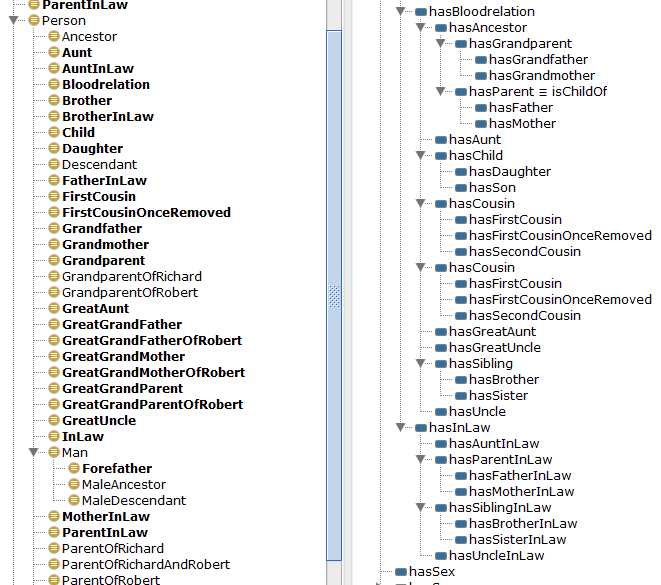
\includegraphics[width=\largefigwidth]{figures/class_prop_hierachy_final}\caption{A part of the class and property hierarchy of the final \fhkb.}\label{fig:class_and_prop_hierachy}
% \end{center}
% \end{figure}


\section{How to use these exercises}

Start at exercise one and work through to the last exercise. Don't just read the exercises and think you know what will happen; actually do it and you'll learn more. 

\pagenumbering{arabic}

\addtocounter{excounter}{1}
\chapter{Exercise \arabic{excounter}}
\addtocounter{excounter}{1}

\steps{Getting things started}{
\item Install \protege.
\item Install the matrix plugin.
\item Open a new ontology called \texttt{fhkb-x.owl}, where x is your student user id.
\item Remember to save your file often while working\ldots
}

\section{Notes}

Your machines in the School have \protege installed. The instructions below are for use `off-site'.

\section{Installing \protege}
Go to \url{http://protege.stanford.edu/download/registered.html} and download the platform independent installer of \protege Desktop 4.X (you do not have to register in order to download the software). Select the appropriate one for your operating system. We recommend downloading it bundled with the Java VM, to ensure compatibility. After the download is completed, run the installer and follow the instructions, selecting the appropriate VM (either the one bundled with it or your default one). 

Once the installation is completed, open \protege and go to File >> Check for plugins. Select the Matrix views plugin, as shown on the screenshot towards the end of this chapter. Click install, wait until the software asks for a restart, close and re-open \protege.

\section{Create a first ontology}
Select File >> Save as, select either RDF/XML or OWL/XML, navigate to your preferred directory and save the file using the name fhkb-x, replacing the x with your student user id (e.g. mbax1234). The extension (*.owl) is put automatically. To be sure, go to File >> Save, and do so frequently during your upcoming modelling efforts, as \protege is known to crash in the unlikeliest situations.

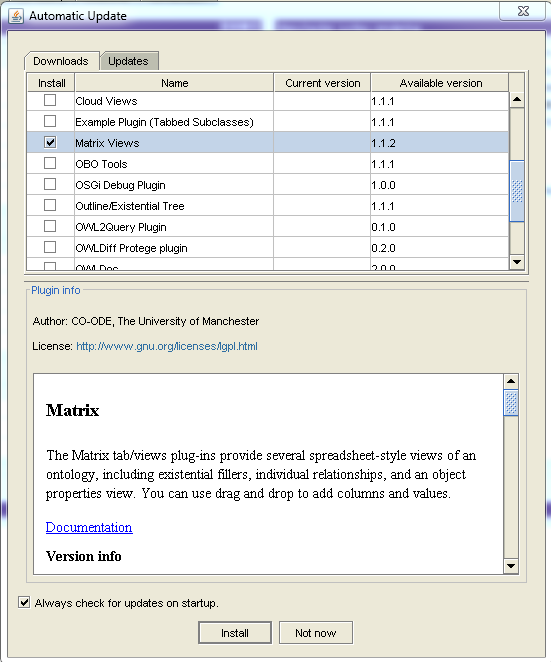
\includegraphics[width=15cm]{images/matrix_install.PNG}
\chapter{Exercise \arabic{excounter}}
\addtocounter{excounter}{1}

\steps{Create individuals}{
\item Load the initial ontology from the course unit home page
  (\url{http://studentnet.cs.manchester.ac.uk/pgt/COMP62342/}) into
  \protege.  
\item Add about 6 more individuals to your \fhkb---use the emboldened names from the table in Appendix~\ref{chap:familydata}; you may add more names if you wish. For each individual, create an IRI fragment with the given names followed by family name, followed by birth year, each separated by underscores. 
\item Create two object properties: \con{hasFather} and \con{hasMother}. Add the appropriate assertions from the data table; run the reasoner.
\item Ask the DL query \con{hasFather value \ids}.
\item Add inverses for the two properties: \con{isFatherOf} and \con{isMotherOf}; run the reasoner.
\item Ask the DL query \con{isMotherOf value \irds} and \con{isMotherOf value \ids}.
}

\chapter{Exercise \arabic{excounter}}
\addtocounter{excounter}{1}

\steps{Create \con{hasParent}}{
\item Add another object property \con{hasParent} and its obvious inverse. Make \con{hasParent} a super-property of \con{hasMother} and \con{hasFather}.
\item Run the reasoner.
\item Ask the DL queries: \con{hasParent value \ids} and \con{hasParent value \imgs}. Ask similar queries using the \con{isParentOf} property.
\item Look at the object hierarchy and see the reasoner maintaining the `is' side of the hierarchy.
\item Write a DL query to find the grandparents of \rds. Specialise that query to find \rds's grandfathers. 
}
\chapter{Exercise \arabic{excounter}}
\addtocounter{excounter}{1}

\steps{Finding ancestors and descendants}{

\item Add the object property  \con{hasAncestor} and make it a super-property of \con{hasParent}.
\item Add its inverse \con{hasDescendant}.
\item Make \con{hasAncestor} transitive.
\item Run the reasoner.
\item Ask the DL queries: \con{hasDescendant value \irds} and  \con{hasAncestor value william\_george\_bright\_1901}. Check the answers against the table in Appendix~\ref{chap:familydata}.
\item Ask more queries and check your answers.
}
\chapter{Exercise \arabic{excounter}}
\addtocounter{excounter}{1}
\herebedragons
\steps{Finding grandparents}{
\item Add the  object properties \con{hasGrandparent}, \con{hasGrandmother} and \con{hasGrandfather} arranged in the obvious hierarchy.
\item Make \con{hasGrandparent} a sub-property of the appropriate property in the growing object hierarchy.
\item Add the obvious `is' inverses.
\item Add a sub-property chain \con{hasParent o hasFather} to the \con{hasGrandfather} property; do the equivalent for \con{hasGrandmother}.
\item Run the reasoner (and look at the object hierarchy).
\item Ask DL queries about grandparents and grandchildren of various people.
\item Add in properties and sub-property chains for finding great grandparents. (you may have to add some more individuals to test these properties.) 
\item Run the reasoner and test with DL queries.
}
\chapter{Exercise \arabic{excounter}}
\addtocounter{excounter}{1}

\steps{Finding all blood relations}{
\item Add the object property \con{hasBloodRelation} to the object property hierarchy.
\item Is this property transitive?
\item What is this property's inverse? It is its own inverse, so make it symmetric.
\item What is the sub-property chain that determines one's blood relations? Add this sub-property chain to \con{hasBloodRelation}.
\item Run the reasoner and test your answer.
\item One good test is to find the blood relations of the person furthest back in the hierarchy; do we get his or her blood relations? How do we fix it? Ask a human being---we don't yet know, in the ontology, that everyone has an ancestor; once we do know this, this sub-property chain will work. We know as humans that everyone has parents; the `computer' doesn't know this yet---see Exercise~\ref{ex_classes}.
\item Look at the object property hierarchy. 
}
\chapter{Exercise \arabic{excounter}}
\addtocounter{excounter}{1}
\label{ex:classes}
\label{ex:sex}

\herebedragons
\steps{Adding classes of individuals}{
\item Add the class \con{Person} to the \fhkb.
\item Add the classes \con{Sex}, \con{Male} and \con{Female}; make \con{Male} and \con{Female} subclasses of \con{Sex}.
\item Add the object property \con{hasSex}; restrict the class \person to \con{hasSex some Sex}.
\item Make two classes \con{Man} and \con{Woman}. Make \man\  \con{EquivalentTo: Person and hasSex some Male} and do the equivalent for \woman.
\item Run the reasoner. %Look to see where \man and \woman are in the class hierarchy; work out why.
\item Ask the DL query \con{Male and Female}; should this be possible? Make \con{Male} and \con{Female} disjoint, run the reasoner  and ask the query again. 
\item Ask the DL query \con{Sex and not (Male or Female)}; the answer suggests that there are other ways of being a \con{Sex} than being either \con{Male} or \con{Female}. Stop this happening by adding the covering axiom \con{Sex EquivalentTo: Male or Female}; run the reasoner and ask the query again.
\item Ask the DL query \con{Sex and not Female}; find an explanation for the results.
\item Ask the DL query \con{Man and Woman}; is it possible for a person to be both a man and a woman (according to our ontology)? Find out why this is possible or not.  
\item Ask the DL query \con{Person and  not (Man or Woman)}, that is, is it possible to be a person and neither a man nor a woman?
\item Ask the DL query \con{Person and not Man}; what do you find out? 
\item Make the object  property \con{hasSex} functional, run the reasoner and do all the queries again. 
\item Ask for an explanation of this inference.
% \item Add the restrictions \con{hasFather some Man} and \con{hasMother some Woman} to \person. Run the reasoner and ask which individuals have a mother. Also ask the DL query for which individuals have a grandmother. Ask for explanations.
% \item Test the \con{hasBloodRelation} property again. This time you should see it working. this is because we've now said everyone has a mother and everyone has a father, therefore everyone has a parent and thus an ancester. If everyone can have an ancestor,  then everyone is someone's descendent. 
}
\chapter{Exercise \arabic{excounter}}
\addtocounter{excounter}{1}

\steps{Domains and ranges}{
\item Run the reasoner and ask DL queries about who is a \man,  \woman and \person; note the answers.
\item  Add the domain \person and range \man to \con{hasFather} and add the domain \person and range \woman to \con{hasMother}.
\item Run the reasoner and inspect the object hierarchy to see what the reasoner has done with the domains and ranges of the other properties; make any changes that are necessary.
\item Ask DL queries about who is a \man,  \woman and \person; note for whom we don't have a specific sex.
\item Write the following defined classes (using the \con{equivalentTo:} construct):
\begin{enumerate}
\item  Parent---All the individuals that are parents.
\item A \con{Grandparent} class that uses the \con{isGrandparentOf} property and \con{Grandparent2} that uses \con{EquivalentTo: Person and (isParentOf some (Person and isParentOf some Person))}. 
\end{enumerate}
Run the reasoner, look to see where the classes are placed in the
hierarchy and work out why.  

\item Add the restrictions \con{hasFather some Man} and \con{hasMother some Woman} to \person. Run the reasoner and ask which individuals have a mother. Also ask the DL query for which individuals have a grandmother. Ask for explanations.
\item Test the \con{hasBloodRelation} property again. This time you should see it working. this is because we've now said everyone has a mother and everyone has a father, therefore everyone has a parent and thus an ancester. If everyone can have an ancestor,  then everyone is someone's descendent. 

}
\chapter{Data Properties in the \fhkb}
\label{chap:data}
 
We now have some individuals with some basic object properties between individuals. \owlii, however, also has data properties that can relate an object or individual to some item of data. There are data about a \person, such as years of events and names etc. So, in this Chapter you will:
\begin{enumerate}
\item Make some data properties to describe event years to people;
\item Create some simple defined classes that group people by when they were born;
\item Try counting the numbers of children people have\ldots
\item Deal with the open world assumption;
\item Add given and family names to individuals in the \fhkb.
\end{enumerate}

\snapshot{There is a snapshot of the ontology as required at this point in the tutorial available at \fhkbhome.}

\section{Adding Some Data Properties for Event Years}

Everyone has a birth year; death year; and some have a marriage year and so on. We can model these simply with data properties and an integer as a filler. \owlii has a DateTime datatype, where it is possible to specify a precise time and date down to a second.\footnote{\url{http://www.w3.org/TR/2008/WD-owl2-quick-reference-20081202/#Built-in_Datatypes_and_Facets}} This proves cumbersome (see \url{http://robertdavidstevens.wordpress.com/2011/05/05/using-the-datetime-data-type-to-describe-birthdays/} for details); all we need is a simple indication of the year in which a person was born. Of course, the integer type has a zero, which the Gregorian calendar for which we use integer as a proxy does not, but integer is sufficient to our needs. Also, there are various ontological treatments  of time and information about people (this extends to names etc. as well), but we gloss over that here---that's another tutorial.

We can have dates for birth, death and (eventually) marriage (see Chapter~\ref{chap:marriage}) and we can just think of these as event years. We can make a little hierarchy of event years as shown in Figure~\ref{fig:data_hierarchy}).

\steps{Create a data property hierarchy}{
\item Create the data property \con{hasEventYear} with range integer and domain \person;
\item Create the data property \con{hasBirthYear} and make it a sub-property of \con{hasEventYear} (that way, the domain and range of \con{hasEventYear} are inherited);
\item Create the data property \con{hasDeathYear} and make it a sub-property of \con{hasEventYear};
\item For each individual add the birth years shown in Table~\ref{tab:familydata} (see appendix). You do not actually have to go back to the table---it is easier to read the birth years simply off the individual names.
}
\snapshot{Again, asserting birth years for all individuals can be a bit tedious. The reader can find a convenience snapshot of the ontology at this stage at \fhkbhome.
}

We now have an ABox with individuals with fact assertions to data indicating a birth year. We can, if we wish, also add a class restriction to the \person class saying that each and every instance of the class \person holds a data property to an integer and that this property is called `hasBirthYear'. As usual when deciding whether to place such a restriction upon a class, ask whether it is true that each and every instance of the class holds that property; this is exactly the same as we did for the object properties in Chapter~\ref{chap:person}. Everyone does have a birth year, even if it is not known.

Once birth years have been added to our individuals, we can start asking some questions. 

\steps{DL queries}{
\item Use a DL query to ask: \begin{itemize}
\item \person born after 1960;
\item \person born in the 1960s;
\item \person born in the 1800s;
\item \person that has fewer than three children;
\item \person that has more than three children.
\end{itemize}
}

The DL query for people born in the 1960s is:
\\\\
\owlcode{
Person and hasBirthYear some int[>= 1960, < 1970]
}

This kind of interval is known as a facet.

\subsection{Counting Numbers of Children}
\label{sec:countchildren}

The last two queries in the list do not work as expected. We have asked, for instance, for \person that have more than three children, but we get no members of \person in the answer, though we know that there are some in the \fhkb (e.g., \ijb). This is because there is not enough information in the \fhkb to tell that this person has more than three \textbf{different} people as children. As humans we can look at the four children of John Bright and know that they are different -- for instance, they all have different birth years. The automated reasoner, however, does not know that a \person can only have one birth year.

\steps{Make a functional object property}{
\item Make the property \con{hasBirthYear} functional. 
\item Ask the query for \person that has more than three children again.
}

This time the query should work. All the other event year properties should be made functional, expect \con{hasEventYear}, as one individual can have many event years. As the children have different birth years and an individual can only hold one \con{hasBirthYear} property, then these people must be distinct entities.

Of course, making birth year functional is not a reliable way of ensuring that the automated reasoner knows that the individual are different. It is possible for two \person to have the same birth year within the same family -- twins and so on. \ipwb has three children, two of which are twins, so will not be a member of the class of people with at least three children. So, we use the \textbf{different individuals} axiom. Most tools, including \protege, have a feature that allows all individuals to be made different.

\steps{Make all individuals different}{
\item Make all individuals different;
\item Ask the above queries again.
}

From now on, every time you add individuals, make sure the different individuals axiom is updated.

\section{The Open World Assumption}

We have met again the open world assumption and its importance in the \fhkb. In the use of the functional characteristic on the \con{hasBirthYear} property, we saw one way of constraining the interpretation of numbers of children. We also introduced the `different individuals' axiom as a way of making all individuals in a knowledge base distinct. There are more questions, however, for which we need more ways of closing down the openness of \owlii.

Take the questions:
\begin{itemize}
\item People that have exactly two children;
\item People that have only brothers;
\item People that have only female children.
\end{itemize}

We can only answer these questions if we locally close the world.\herebedragons  We have said that David and Margaret have two children, Richard and Robert, but we have not said that there are not any others. As usual, try not to apply your domain knowledge too much; ask yourself what the automated reasoner actually knows. As we have the open world assumption, the reasoner will assume, unless otherwise said, that there could be more children; it simply doesn't know.

Think of a railway journey enquiry system. If I ask a standard closed world system about the possible routes by rail, between Manchester and Buenos Aires, the answer will be 'none', as there are none described in the system. With the open world assumption, if there is no information in the system then the answer to the same question will simply be `I don't know'. We have to explicitly say that there is no railway route from Manchester to Buenos Aires for the right answer to come back.

We have to do the same thing in OWL. We have to say that David and Margaret have only two children. We do this with a \textbf{type assertion} on individuals . So far we have only used fact assertions. A type assertion to close down \ds' parentage looks like this:
\\\\
\owlcode{
isParentOf only \{\irds, \irjs\}
}

This has the same meaning as the closure axioms that you should be familiar with on classes. We are saying that the only fillers that can appear on the right-hand-side of the \con{isParentOf} property on this individual are the two individuals for Richard and Robert. We use the braces to represent the set of these two individuals.\herebedragons

\steps{Make a closure axiom}{
\item Add the closure assertion above to \ds;
\item Issue the DL query \con{isParentOf exactly 2 Person}.
}

The last query should return the answer of \ds. Closing down the whole \fhkb ABox is a chore and would really have to be done programmatically. OWL scripting languages such as the Ontology Preprocessing Language\footnote{\url{http://oppl2.sourceforge.net}} (OPPL)~\cite{oppl} can help here. Also going directly to the OWL API~\cite{owlapi}\footnote{\url{http://owlapi.sourceforge.net/}}, if you know what you are doing, is another route. 
\\\\
\dragon{Adding all these closure type assertions can slow down the reasoner; so think about the needs of your system -- just adding it `because it is right' is not necessarily the right route.}


%\comment{the K-operator}

%\rds has only one father, but \ds may have any old nubmer of children; how do we close it?

\section{Adding Given and Family Names}

We also want to add some other useful data facts to people -- their names. We have been putting names as part of labels on individuals, but data fact assertions make sense to separate out family and given names so that we can ask questions such as `give me all people with the family name Bright and the first given name of either James or William'. A person's name is a fact about that person and is more, in this case, than just a label of the representation of that person. So, we want family names and given names. A person may have more than one given name -- `Robert David', for instance -- and an arbitrary number of given names can be held. For the \fhkb, we have simply created two data properties of \con{hasFirstGivenName} and \con{hasSecondGivenName}). Ideally, it would be good to have some index on the property to given name position, but OWL has no n-ary relationships. Otherwise, we could reify the \con{hasGivenName} property into a class of objects, such as the following:
\\\\
\owlcode{
Class: GivenName

SubClassOf:hasValue some String,

	hasPosition some Integer
}
\\\\
\noindent but it is really rather too much trouble for the resulting query potential.

As already shown, we will use data properties relating instances of \person to strings. We want to distinguish family and given names, and then different positions of given names through simple conflating of position into the property name. Figure~\ref{fig:data_hierarchy} shows the intended data property hierarchy.

\begin{figure}
\begin{center}
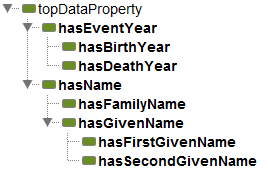
\includegraphics[width=\figwidth]{figures/new/event_name_hierarchy.PNG}\caption{The event year and name data property hierarchies in the \fhkb.}\label{fig:data_hierarchy}
\end{center}
\end{figure}

Do the following:
\steps{Data properties}{
\item Create the data properties as described in Figure~\ref{fig:data_hierarchy};
\item Give the \con{hasName} property the domain of \person and the range of \con{String};
\item Make the leaf properties of given names functional;
\item Add the names shown in Table~\ref{tab:familydata} (appendix); Again, it may be easier to read the names of the individual names.
\item Ask the questions:
\subitem all the people with the first given name `James';
\subitem all the people with the first given name `William';
\item All the people with the given name `William';
\item All the people with the given name `William' and the family name `Bright'.
}

The name data property hierarchy and the queries using those properties displays what now should be familiar.
Sub-properties that imply the super-property. So, when we ask \con{hasFirstGivenName value "William"} and then the query \con{hasGivenName value value "William"} we can expect different answers. There are people with `William' as either first or second given name and asking the question with the super-property for given names will collect both first and second given names.

\section{Summary}

We have used data properties that link objects to data such as string, integer, floats and Booleans etc. OWL uses the XML data types. We have seen a simple use of data properties to simulate birth years. The full \fhkb also uses them to place names (given and family) on individuals as strings. This means one can ask for the \person with the given name "James", of which there are many in the \fhkb.

Most importantly we have re-visited the open world assumption and its implications for querying an OWL ABox. We have looked at ways in which the ABox can be closed down -- unreliably via the functional characteristic (in this particular case) and more generally via type assertions.

All the DL queries used in this chapter can also serve as defined classes in the TBox. It is a useful exercise to progressively add more defined classes to the \fhkb TBox. Make more complex queries, make them into defined classes and inspect where they appear in the class hierarchy. 
\\
\expressivity{SROIQ(D)}

\ctime{1891157}{1134}{201}

\note{Note that we now cover the whole range of expressivity of OWL~2. HermiT at least is impossibly slow by now. This may be because HermiT does more work than the others. For now, we recommend to use either Pellet or FaCT++.}
\chapter{Exercise \arabic{excounter}}
\addtocounter{excounter}{1}
\herebedragons
\steps{Finding siblings}{
\item Add an object property \con{hasSibling} at the appropriate place to the object property hierarchy.
\item Decide whether it is symmetric  and/or transitive.
\item Add the property chain that will find siblings.
\item Run the reasoner.
\item Ask the DL query \con{hasSibling value \irds}; what's the problem?
\item Make \con{hasSibling} irreflexive, this should make it impossible for \rds to be his own brother. What happens? ask for an explanation (from a human being).
\item Add two sub-properties for \con{hasSibling}: \con{hasBrother} and \con{hasSister}. Decide on the transitivity, symmetry etc. for these properties and add an inverse property if you think it appropriate.
\item What sub-property chains do we need to make \con{hasBrother} work? Remember that we do not, as yet, know the sex of \rds and several other individuals.
\item The \con{isFatherOf} property has a range of \person; this will not determine the sex of a father's child. To fix this, make a property hierarchy of \con{hasChild}, \con{hasSon} and \con{hasDaughter}; add the appropriate domains and ranges.
\item Use an \con{EquivalentProperty} axiom to tie \con{hasChild} to an appropriate existing object property.
\item Add \con{hasSon} and \con{hasDaughter} assertions to the individuals.
\item Add sub-property chains to \con{hasBrother} and \con{hasSister} using these new properties; run the reasoner and test the answers with DL queries.
\item Inspect the object hierarchy.
}
\chapter{Exercise \arabic{excounter}}
\addtocounter{excounter}{1}

\steps{Finding aunts and uncles}{
\item Add the object properties \con{hasUncle} and \con{hasAunt}, their domains, ranges and inverses at the appropriate place in the object hierarchy.
\item An uncle is a parent's brother (that is, a blood relation, not an `uncle-in-law); add a sub-property chain to find uncles and a similar one to find aunts.
\item Run the reasoner and test with DL queries. \rds's uncles are John Bright and Peter William Bright; his aunt is Eileen Reever.
}
\chapter{Cousins in the \fhkb}
\label{chap:cousins}
\taskstart 

In this Chapter you will
\begin{enumerate}
\item Revise or get to know about degrees and removes of cousin;
\item Add the properties and sub-property chains for first and second cousins;
\item Add properties and sub-property chains for some removes of cousins;
\item Find out that the siblings debacle haunts us still;
\item Add a defined class that does first cousins properly.
\end{enumerate}

\snapshot{There is a snapshot of the ontology as required at this point in the tutorial available at \fhkbhome.}

\dragon{Be warned; from here on the reasoner can start running slowly! Please see warning at the beginning of the last chapter for more information.}

\section{Introducing Cousins}
\label{sec:cousin_intro}

Cousins can be confusing, but here is a brief summary:
\begin{itemize}
\item First cousins share a grandparent, but are not siblings;
\item Second cousins share a great grandparent, but are not first cousins or siblings;
\item Degrees such as first and second cousin give the distance to the nearest common ancestor;
\item Removes give differences in generation. So, my Dad's first cousins (his generation) are my (\rds's) first cousins once removed.
\end{itemize}
Simply, my first cousins are my parent's sibling's children. As usual, we can think about the objects and put in place some sub-property chains.

\section{First Cousins}

Figure~\ref{fig:first_cousins} shows the sub-property chain for first cousins. As usual, think at the object level; to get to the first cousins of \rds, we go to the parents of \rds, to their siblings and then to their children. We go up, along and down. The OWL for this could be:

\owlcode{
ObjectProperty: hasFirstCousin

    SubPropertyOf: 
        hasCousin
    
    SubPropertyChain: 
        hasParent o hasSibling o hasChild
    
    Characteristics: 
        Symmetric
}

\begin{figure}
\begin{center}
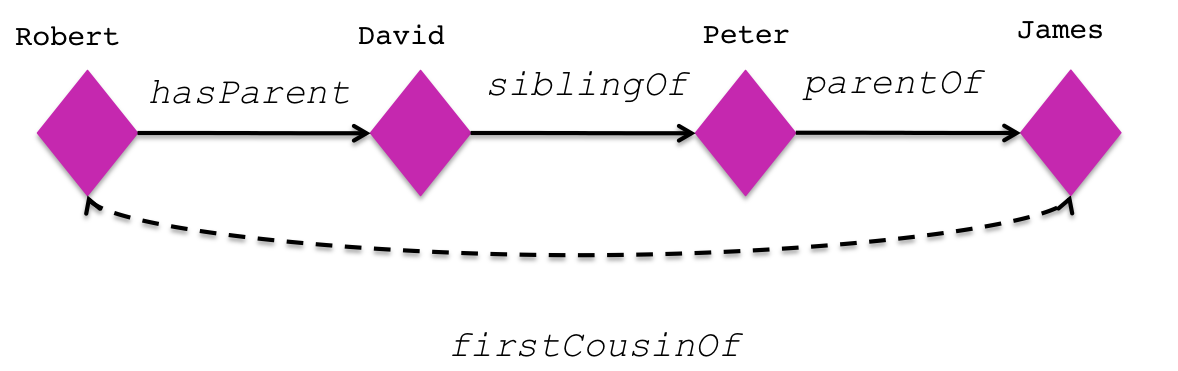
\includegraphics[width=\figwidth]{figures/cousin}
\caption{Tracing out the sub-property chain for cousins going from a child to a parent, to its sibling, and down to its child, a cousin}
\label{fig:first_cousins}
\end{center}
\end{figure}

Note that we follow the definitions in Section~\ref{sec:cousin_intro} of first cousins sharing a grandparent, but not a parent. The sub-property chain goes up to children of a grandparent (a given person's parents), along to siblings and down to their children. We do not want this property to be transitive. One's cousins are not necessarily my cousins. The blood uncles of \rds have children that are his cousins. These first cousins, however, also have a mother that is not a blood relation of \rds and the mother's sibling's children are not cousins of \rds.  

We do, however, want the property to be symmetric. One's cousins have one's-self as a cousin.

We need to place the cousin properties in the growing object property hierarchy. Cousins are obviously blood relations, but not ancestors, so they go off to one side, underneath \con{hasBloodrelation}. We should group the different removes and degree of cousin underneath one \con{hasCousin} property and this we will do.

Do the following:
\steps{First cousins}{
\item Add the property of \con{hasCousin} to the hierarchy underneath \con{hasBloodrelation};
\item Add \con{hasFirstCousin} underneath this property;
\item Add the sub-property chain as described above;
\item Run the reasoner and look at the first cousins of \rds.
}

You should see the following people as first cousins of \rds: Mark Anthony Heath, Nicholas Charles Heath, Mark Bright, Ian Bright, Janet Bright, William Bright, James Bright, Julie Bright, Clare Bright, Richard John Bright and Robert David Bright. The last two, as should be expected, are first cousins of \rds and this is not correct. As \ds will be his own brother, his children are his own nieces and nephews and thus the cousins of his own children. Our inability to infer siblings correctly in the \fhkb haunts us still and will continue to do so.

\dragon{Although the last query for the cousins of \rds should return the same results for every reasoner, we have had experiences where the results differ.}

\section{Other Degrees and Removes of Cousin}

Other degrees of cousins follow the same pattern as for first cousins; we go up, along and down. For second cousins we go up from a given individual to children of a great grandparent, along to their siblings and down to their grandchildren. The following object property declaration is for second cousins (note it uses the \con{isGrandparentOf} and its inverse properties, though the parent properties could be used) :

\owlcode{
ObjectProperty: hasSecondCousin

    SubPropertyOf: 
        hasCousin
    
    SubPropertyChain: 
        hasGrandParent o hasSibling o isGrandParentOf
    
    Characteristics: 
        Symmetric
}

`\emph{Removes}' simply add in another `leg' of either `up' or `down' either side of the `along'---that is, think of the actual individuals involved and draw a little picture of blobs and lines---then trace your finger up, along and down to work out the sub-property chain. The following object property declaration does it for first cousins once removed (note that this has been done by putting this extra `leg' on to the \con{hasFirstCousin} property; the symmetry of the property makes it work either way around so that a given person is the first cousin once removed of his/her first cousins once removed): 
\\\\
\owlcode{
ObjectProperty: hasFirstCousinOnceRemoved

    SubPropertyOf: 
        hasCousin
    
    SubPropertyChain: 
        hasFirstCousin o hasChild
    
    Characteristics: 
        Symmetric
}
\\\\
To exercise the cousin properties do the following:
\steps{Cousin properties}{
\item Add properties for second degree cousins;
\item Add removes for first and second degree cousins;
\item Run the reasoner and check what we know about \rds' other types of cousin.
}
You should see that we see some peculiar inferences about \rds' cousins -- not only are his brother and himself his own cousins, but so are his father, mother, uncles and so on. This makes sense if we look at the general sibling problem, but also it helps to just trace the paths around. If we go up from one of \rds' true first cousins to a grandparent and down one parent relationship, we follow the first cousin once removed path and get to one of \rds' parents or uncles. This is not to be expected and we need a tighter definition that goes beyond sub-property chains so that we can exclude some implications from the \fhkb.
%\todo{check and finish}

\section{Doing First Cousins Properly}

As far as inferring first cousin facts for \rds, we have failed. More precisely, we have recalled all \rds's cousins, but the precision is not what we would desire. What we can do is ask for \rds' cousins, but then remove the children of \rds' parents. The following DL query achieves this:

\owlcode{
Person that hasFirstCousin value \irds 

and (not (hasFather value \ids) or not (hasMother value \imgs)
}
\\
This works, but only for a named individual. We could make a defined class for this query; we could also make a defined class \con{FirstCousin}, but it is not of much utility. We would have to make sure that people whose parents are not known to have siblings with children are excluded. That is, people are not `first cousins' whose only first cousins are themselves and their siblings. The following class does this:

\owlcode{
Class: FirstCousin

EquivalentTo: Person
	that hasFirstCousin some Person
}

\steps{Roberts first cousins}{
\item Make a defined class \con{FirstCousin} as shown above;
\item Make a defined class \con{FirstCousinOfRobert};
\item Create a DL query that looks at \irds first cousins and takes away the children of \irds' parents as shown above.
}
This gives some practice with negation. One is making a class and then `taking' some of it away -- `these, but not those'.\herebedragons 
%\todo{perhaps a bit ore about negation?}

\section{Summary}

We have now expanded the \fhkb to include most blood relationships. We have also found that cousins are hard to capture just using object properties and sub-property chains. Our broken sibling inferences mean that we have too many cousins inferred at the instance level. We can get cousins right at the class level by using our inference based cousins, then excluding some using negation. Perhaps not neat, but it works.

We have reinforced that we can just add more and more relationships to individuals by just adding more properties to our \fhkb object property hierarchy and adding more sub-property chains that use the object properties we have built up upon parentage and sibling properties; this is as it should be.
\\

\expressivity{SROIQ(D)}

\ctime{0}{111395}{868}
%\chapter{Exercise \arabic{excounter}}
\addtocounter{excounter}{1}

\steps{Individuals in class expression: Nominals}{
\item blah blah
}
\chapter{Exercise \arabic{excounter}}
\addtocounter{excounter}{1}

\steps{In-laws: Modelling partnerships}{
\item Add the class \con{Partnership} to the \fhkb as a sibling of \person and make it disjoint with its primitive siblings.
\item Create the object properties \con{hasParticipant}, \con{hasMaleParticipant} and \con{hasFemaleParticipant} in the obvious object hierarchy, along with their inverses. \con{Partnership} is their common domain and add the obvious ranges to these properties.
\item Add a restriction of \con{hasParticipant min 2 Person} to the \con{Marriage} class.
\item Create the object properties \con{hasSpouse}, \con{hasWife} and \con{hasHusband} and inverses where appropriate (or use property characteristics when they are not). Use sub-property chains to infer when two individuals are husband and wife. \ds and \mgs were married in 1958; create an individual for this marriage (you can add a \con{hasMarriageYear} data property if you wish). John Bright and Joyce Gosport were married in 1954. Add another individual for this marriage.
\item Run the reasoner and ask DL queries to test what you have done.
\item Create new object properties for in-laws-brother-in-law, sister-in-law (hint: these last two have possible sub-property chains)  and sibling-in-law. You can also now add properties to find uncles- and aunts-in-law.
\item Run the reasoner, and ask DL queries to confirm that it all works.
\item Add these  two property hierarchies to the main object property hierarchy, reason and look at it.
}
\chapter{Exercise \arabic{excounter}}
\addtocounter{excounter}{1}
\herebedragons
\steps{Finding parents with only sons}{
\item Ask the DL query \con{isParentOf some Man}; note the answer.
\item The query finds someone that has at least one son; we want a query that asks for  people that are parents of only sons.
\item Ask the DL query \con{isParentOf only Man}; note the answer. Are there any unusual answers?
\item We need to `close off' what people individuals are parents of. For \ds we do this with an axiom such as \con{isParentOf only \{\irjs, \irds\}}. Add such axioms to your \fhkb's individuals (\ds, for instance, should have such an axiom.)   and ask the questions again, noting the answers.  (note how fast the reasoner runs.)
\item Now write a defined class \con{ParentOfOnlySons}. this will be something like:

\con{EquivalentTo:  Person and isParentOf some Man and isParentOf only Man}.

\item Run the reasoner; where is the class placed in the TBox; which individuals are members of this class? 
}
\chapter{Exercise \arabic{excounter}}
\addtocounter{excounter}{1}
\herebedragons
\steps{Are sibling's grandparents the same?}{
\item Make two defined classes \con{GrandparentOfRobert} and \con{GrandparentOfRichard}. Use the pattern \con{Person and EquivalentTo: isParentOf some (Person and isParentOf value x)} where x is either \irds or \irjs.
\item Run the reasoner and find out if the two classes are found to be equivalent; they won't be, despite the fact \rds and \rjs share parents and therefore share the same grandparents.
\item It doesn't work. If you add \con{hasParent max 2 Person} as a restriction to the class \person (only as a necessary condition), re-run the reasoner, then everything will work. You'll see that the two classes have been inferred to be equivalent.
\item It's all to do with openness; ask a human being or read the full \fhkb manual.
 
}
\chapter{Exercise \arabic{excounter}}
\addtocounter{excounter}{1}
\herebedragons
\steps{Grandparent as a defined class}{
\item Make the class \con{Parent} as \con{EquivalentTo:  Person  and isParentOf some Person}.
\item Make two defined classes, \con{Grandparent1} and \con{Grandparent2};  in one use the \con{isGrandparentOf} property and in the other use \con{isParentOf some (Person and isParentOf some Person)}.
\item Run the reasoner  and look at the class hierarchy. Do both classes appear as subclasses of \con{Parent} as they should (all grandparents are, by definition, parents) and are they equivalent? think about it.
}
\chapter{Exercise \arabic{excounter}}
\addtocounter{excounter}{1}
\herebedragons
\steps{Making a big class hierarchy}{
\item Add defined classes for the following (some may already exist):
\begin{itemize}
\item Son and Daughter;
\item Brother and Sister;
\item Cousin, FirstCousin, SecondCousin, FirstCousinOnceRemoved (and so on until you get bored);
\item InLaw, MotherInLaw, FatherInLaw and so on;
\item Aunt, Uncle, UncleInLaw, and so on;
\item GrandParent, Grandfather, GreatGrandparent, and so on; 
\end{itemize}
\item Look at how the class hierarchy grows; its shape and any `unusual' placements; use explanation widely to check on your growing hierarchy.
\item Note what happens to the classes \con{Son} and \con{Daughter} in the hierarchy---why?
}

\appendix
%\chapter{Property Characteristics}
\label{chap:char}

This appendix illustrates each of OWL's property characteristics.

\section{Functional}

\section{Transitive}

\section{Reflexive}

\section{Irreflexive}


\section{Symmetric}
.
\chapter{FHKB Family Data}
\label{chap:familydata}
\begin{landscape}
\begingroup
\small
\begin{longtable}{lp{2cm}p{2cm}lp{2cm}ll}
\caption{The list of individuals in the FHKB}\\
\label{tab:familydata}
%\textbf{Person} & First given name & Second given name & Family name & Birth year & Mother & Father \\ \hline
\endhead
\hline \multicolumn{7}{l}{\emph{continued..}}
\endfoot
\endlastfoot
\textbf{Person} & First given name & Second given name & Family name & Birth year & Mother & Father \\ \hline
Alec John Archer 1927 & Alec & John & Archer & 1927 & Violet Heath 1887  & James Alexander Archer 1882  \\
\textbf{Charles Herbert Rever 1895} & Charles & Herbert & Rever & 1895 & Elizabeth Frances Jessop 1869  & William Rever 1870  \\
Charlotte Caroline Jane Bright 1894 & Charlotte & Caroline Jane & Bright & 1894 & Charlotte Hewett 1863 & Henry Edmund Bright 1862 \\
Charlotte Hewett 1863 & Charlotte & none & Hewett & 1863 & not specified & not specified \\
\textbf{Clare Bright 1966} & Clare & none & Bright & 1966 & Diana Pool & Peter William Bright 1941  \\
Diana Pool & Diana & none & Pool & none & not specified & not specified  \\
\textbf{David Bright 1934} & David & none & Bright & 1934 & Iris Ellen Archer 1906  & William George Bright 1901  \\
Dereck Heath & Dereck & none & Heath & 1927 & not specified & not specified \\
\textbf{Eileen Mary Rever 1929} & Eileen & Mary & Rever & 1929 & Violet Sylvia Steward 1894  & Charles Herbert Rever 1895  \\
Elizabeth Frances Jessop 1869 & Elizabeth & Frances & Jessop & 1869 & not specified & not specified \\
Ethel Archer 1912 & Ethel & none & Archer & 1912 & Violet Heath 1887  & James Alexander Archer 1882  \\
Frederick Herbert Bright 1889 & Frederick & Herbert & Bright & 1889 & Charlotte Hewett 1863  & Henry Edmund Bright 1862  \\
Henry Edmund Bright 1862 & Henry & Edmund & Bright & 1862 & not specified & not specified \\
Henry Edmund Bright 1887 & Henry & Edmund & Bright & 1887 & Charlotte Hewett 1863  & Henry Edmund Bright 1862  \\
\textbf{Ian Bright 1959} & Ian & none & Bright & 1959 & Joyce Gosport & John Bright 1930  \\
\textbf{Iris Ellen Archer 1906} & Iris & Ellen & Archer & 1906 & Violet Heath 1887  & James Alexander Archer 1882  \\
James Alexander Archer 1882 & James & Alexander & Archer & 1882 & not specified & not specified \\
\textbf{James Bright 1964} & James & none & Bright & 1964 & Diana Pool & Peter William Bright 1941  \\
James Frank Hayden Bright 1891 & James & Frank & Bright & 1891 & Charlotte Hewett 1863  & Henry Edmund Bright 1862  \\
\textbf{Janet Bright 1964} & Janet & none & Bright & 1964 & Joyce Gosport & John Bright 1930  \\
\textbf{John Bright 1930} & John & none & Bright & 1930 & Iris Ellen Archer 1906  & William George Bright 1901  \\
John Tacey Steward 1873 & John & Tacey & Steward & 1873 & not specified & not specified \\
Joyce Archer 1921 & Joyce & none & Archer & 1921 & Violet Heath 1887  & James Alexander Archer 1882  \\
Joyce Gosport & Joyce & none & Gosport & not specified & not specified  & not specified  \\
\textbf{Julie Bright 1966} & Julie & none & Bright & 1966 & Diana Pool & Peter William Bright 1941  \\
Kathleen Minnie Bright 1904 & Kathleen & Minnie & Bright & 1904 & Charlotte Hewett 1863  & Henry Edmund Bright 1862  \\
Leonard John Bright 1890 & Leonard & John & Bright & 1890 & Charlotte Hewett 1863 & Henry Edmund Bright 1862  \\
Lois Green 1871 & Lois & none & Green & 1871 & not specified & not specified \\
\textbf{Margaret Grace Rever 1934} & Margaret & Grace & Rever & 1934 & Violet Sylvia Steward 1894  & Charles Herbert Rever 1895  \\
\textbf{Mark Anthony Heath 1960} & Mark & Anthony & Heath & 1960 & Eileen Mary Rever 1929  & Dereck Heath \\
\textbf{Mark Bright 1956} & Mark & none & Bright & 1956 & Joyce Gosport & John Bright 1930  \\
\textbf{Nicholas Charles Heath} 1964 & Nicholas & Charles & Heath & 1964 & Eileen Mary Rever 1929  & Dereck Heath \\
Nora Ada Bright 1899 & Nora & Ada & Bright & 1899 & Charlotte Hewett 1863  & Henry Edmund Bright 1862  \\
Norman James Archer 1909 & Norman & James & Archer & 1909 & Violet Heath 1887  & James Alexander Archer 1882  \\
\textbf{Peter William Bright 1941} & Peter & William & Bright & 1941 & Iris Ellen Archer 1906  & William George Bright 1901  \\
\textbf{Richard John Bright 1962} & Richard & John & Bright & 1962 & Margaret Grace Rever 1934 & David Bright 1934  \\
\textbf{Robert David Bright 1965} & Robert & David & Bright & 1965 & Margaret Grace Rever 1934 & David Bright 1934  \\
Violet Heath 1887 & Violet & none & Heath & 1887 & not specified & not specified \\
\textbf{Violet Sylvia Steward 1894} & Violet & Sylvia & Steward & 1894 & Lois Green 1871  & John Tacey Steward 1873  \\
\textbf{William Bright 1970} & William & none & Bright & 1970 & Joyce Gosport & John Bright 1930  \\
\textbf{William George Bright 1901} & William & George & Bright & 1901 & Charlotte Hewett 1863  & Henry Edmund Bright 1862  \\
William Rever 1870 & William & none & Rever & 1870 & not specified & not specified \\
\end{longtable}
\endgroup
\end{landscape}
\normalsize

%\bibliographystyle{plain}
%\bibliography{fhkb}
\end{document}
